
\vspace{-0.5cm}
\section*{Results}
\vspace{-0.5cm}

In both anisotropic and tuned anisotropic networks, reciprocally connected pairs occur more often than in a random network with the same connection density (Fig.~\ref{fig:2neuron1}A).

\begin{center}\vspace{0.01cm}
  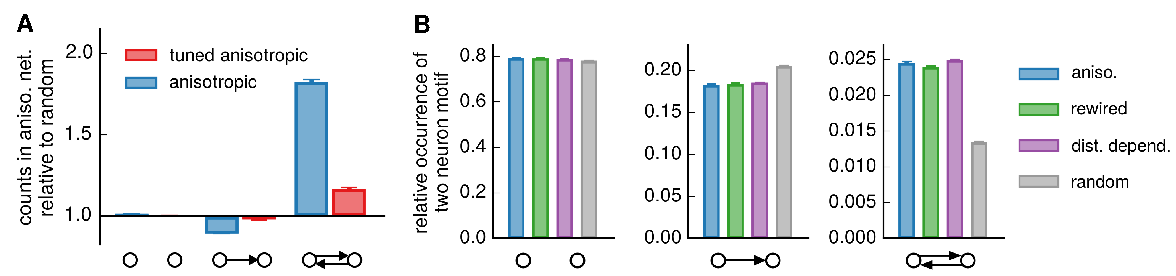
\includegraphics[width=\columnwidth]{%
    /home/fh/sci/rsc/aniso_netw/pub/arxiv18/figures/two_neuron_connections/two_neuron_figure_part1.pdf}
  \captionof{figure}{Unconnected, unidirectional and bidirectional neuron pair occurrences in the network models}
  \label{fig:2neuron1}
\end{center}\vspace{2cm}

However, is this due to anisotropy? Indeed, we find almost identical pair counts in rewired and distance-dependent networks (Fig.~\ref{fig:2neuron1}B). The overrepresentation of reciprocal connections in the data of Perin et al.~\cite{Perin2011} is not explained by distance-dependency (Fig.~\ref{fig:2neuron2}), so that there could be other pair-symmetric irregularities in the connection probabilities that cause the overrepresentation \cite{Hoffmann2017}.

\begin{center}\vspace{0.01cm}
  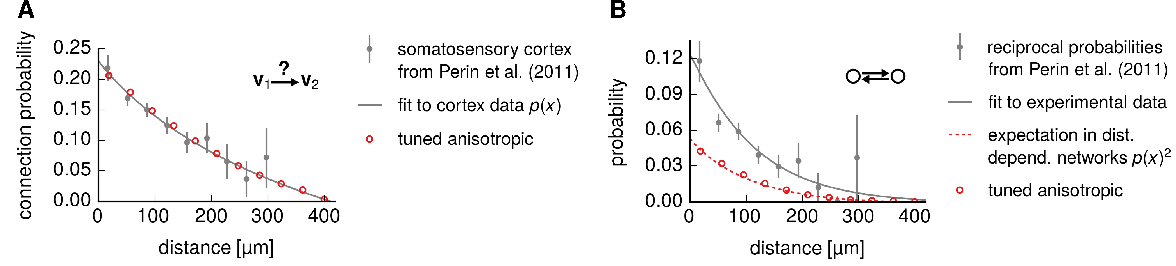
\includegraphics[width=\columnwidth]{%
    /home/fh/sci/rsc/aniso_netw/pub/arxiv18/figures/two_neuron_connections/two_neuron_figure_part2.pdf}
  \captionof{figure}{Some caption}
  \label{fig:2neuron2}
\end{center}\vspace{2cm}

Next we tested the occurrence of three neuron patterns as reported in \cite{Song2005}. We found . Motifs 4, 10, 12 and 14 were also reported in \cite{Perin2011} to be overrepresented.



\begin{center}\vspace{0.01cm}
  \includegraphics[width=\columnwidth]{%
    /home/fh/sci/lab/aniso_netw/ploscb_18/fig/main/fig4_three_motifs.png}
  \captionof{figure}{Spike-timing dependent plasticity changes synaptic efficacies additively, while synaptic normalization acts multiplicatively on the synaptic weights.}
  \label{fig:spines}
\end{center}\vspace{2cm}





\begin{center}\vspace{0.01cm}
  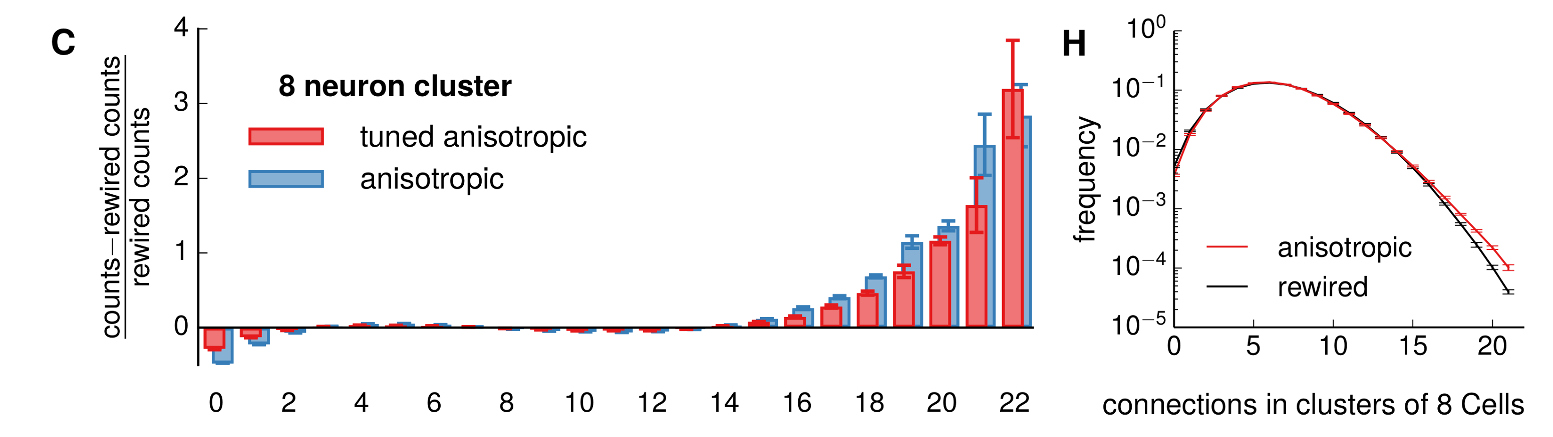
\includegraphics[width=\columnwidth]{%
    figures/new2.png}
  \captionof{figure}{Spike-timing dependent plasticity changes synaptic efficacies additively, while synaptic normalization acts multiplicatively on the synaptic weights.}
  \label{fig:spines}
\end{center}\vspace{2cm}


\begin{center}\vspace{0.01cm}
  \includegraphics[width=0.8\columnwidth]{%
    /home/fh/pub/posters/18_BCCN/poster/figures/cb.png}
  \captionof{figure}{Spike-timing dependent plasticity changes synaptic efficacies additively, while synaptic normalization acts multiplicatively on the synaptic weights.}
  \label{fig:spines}
\end{center}\vspace{2cm}





